\newpage
\section{Análisis Geopolítico de Internet Satelital}
\subsection{La nueva carrera geopolítica en el espacio.}
En las últimas décadas, el internet satelital ha dejado de ser únicamente una solución para brindar conectividad en zonas rurales o de difícil acceso, para convertirse en un elemento estratégico dentro de la competencia tecnológica, económica y política entre las principales potencias del mundo. El desarrollo de satélites de comunicaciones y de grandes constelaciones en órbita terrestre ha transformado la manera en que los países garantizan el acceso a la información, fortalecen su seguridad nacional y amplían su influencia sobre otras regiones.

Actualmente, el liderazgo del internet satelital está concentrado en un reducido grupo de países que poseen la capacidad tecnológica y financiera para diseñar, fabricar, lanzar y operar satélites de comunicaciones. Estados Unidos ocupa una posición predominante gracias a empresas como HughesNet, Viasat y Starlink, que lideran la innovación y la expansión global de este servicio. En Europa, Francia se ha consolidado como un actor relevante mediante Eutelsat, empresa que, tras su integración con OneWeb, fortaleció la presencia europea en el mercado mundial del internet satelital. Por su parte, Japón representa el liderazgo asiático a través de Sky Perfect JSAT, mientras que China impulsa su crecimiento con China Satcom y el desarrollo de nuevas constelaciones satelitales de alcance global. Rusia también mantiene una participación estratégica mediante Gazprom Space Systems, enfocada en garantizar la conectividad de su extenso territorio y de regiones bajo su influencia.

La creciente competencia entre estas empresas y sus países de origen refleja que el internet satelital ya no constituye únicamente un servicio de telecomunicaciones, sino un instrumento de poder geopolítico. La capacidad de ofrecer conectividad global influye en aspectos económicos, militares, científicos y diplomáticos, permitiendo a los Estados fortalecer su soberanía tecnológica y ampliar su presencia internacional. En este contexto, el análisis geopolítico del internet satelital resulta fundamental para comprender cómo las potencias mundiales utilizan esta tecnología como una herramienta de desarrollo, seguridad y liderazgo estratégico en el siglo XXI.




\subsection{Bloque de Estados Unidos “Choque de gigantes privados”}
\subsubsection*{Starlink}
 
Entre todos los proyectos existentes, Starlink, desarrollado por la empresa estadounidense SpaceX, representa el mayor avance tecnológico en materia de conectividad global mediante satélites de órbita baja (LEO). Desde el lanzamiento de sus primeros satélites en 2019, Starlink ha transformado el modelo tradicional de las telecomunicaciones al ofrecer acceso a Internet de alta velocidad en regiones donde las redes terrestres convencionales son limitadas o inexistentes.
 
A diferencia de las redes terrestres convencionales, Starlink utiliza una constelación compuesta por miles de satélites en órbita baja, lo que reduce considerablemente la latencia y mejora la velocidad de transmisión de datos. Este modelo ha permitido que Estados Unidos consolide su liderazgo en el desarrollo de tecnologías espaciales aplicadas a las telecomunicaciones.
\begin{figure}[ht]
    \centering
    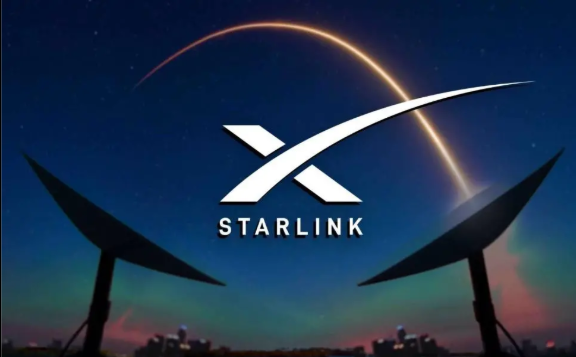
\includegraphics[width=0.7\textwidth]{imagenes/starlink.png}
    \caption{\small\textit{Logo de la empresa más grande de E.E.U.U. Starlink}}
    \label{fig:starlink}
\end{figure}

Estados Unidos mantiene actualmente el liderazgo mundial en internet satelital gracias a la capacidad tecnológica de SpaceX y a la rápida expansión de Starlink. La empresa ha desarrollado la mayor constelación de satélites operativa del mundo, permitiéndole ofrecer cobertura en gran parte del planeta.

Este liderazgo se sustenta en diversos factores:

\begin{itemize}
    \item Desarrollo continuo de tecnologías espaciales innovadoras.
    \item Capacidad para fabricar y lanzar satélites de forma masiva.
    \item Uso de cohetes reutilizables que reducen significativamente los costos de lanzamiento.
    \item Expansión acelerada hacia nuevos mercados internacionales.
    \item Integración entre la industria privada y el desarrollo tecnológico estadounidense.
\end{itemize}
Como resultado, Estados Unidos no solo lidera el mercado del internet satelital, sino que también marca el ritmo del desarrollo tecnológico mundial en este sector.
\subsubsection*{Desafíos internacionales}

A pesar de su liderazgo, Starlink enfrenta diversos desafíos relacionados con las regulaciones impuestas por cada país, la competencia con otros operadores satelitales y las preocupaciones sobre la congestión orbital y la generación de basura espacial. También existen debates sobre la dependencia de una empresa privada para brindar un servicio considerado cada vez más estratégico para la economía y la seguridad internacional.

Entre ellos destacan:

\begin{itemize}
    \item la creciente competencia internacional;
    \item la regulación del uso del espacio ultraterrestre;
    \item la gestión de la basura espacial;
    \item la congestión de las órbitas bajas;
    \item la coordinación del espectro radioeléctrico;
    \item los debates sobre soberanía digital y dependencia tecnológica.
\end{itemize}

\subsubsection*{Proyecto Kuiper (ahora Amazon Leo): la respuesta de Amazon a Starlink}

\noindent\textbf{Qué es y origen}\\

El Proyecto Kuiper es la constelación de internet satelital desarrollada por Amazon, gestionada a través de una filial establecida en 2019. El nombre "Kuiper" era un nombre en código inspirado en el cinturón de Kuiper del sistema solar exterior. Amazon inició la investigación y el desarrollo en 2018, y en julio de 2020 la FCC le otorgó la licencia para desplegar y operar la constelación, bajo la condición de que no interfiriera con proyectos satelitales previamente autorizados.

\subsection{Bloque de China “El Gran Cortafuego”}
\subsection{Bloque Europea “Búsqueda de la autonomía Soberana”}
\subsection{La militarización de los espacios con satélites}
\subsection{La revolución del “Direct-to-Cell”}
